\documentclass[11pt]{article}
\newcommand{\name}{Bill Jin} % PUT YOUR NAME HERE
\usepackage[paper=letterpaper,margin=1in]{geometry}
\usepackage[parfill]{parskip}
\usepackage{amsmath}
\usepackage{fancyvrb}
\usepackage{fancyhdr}
\pagestyle{fancy}
\fancyhf{}
\rhead{\name{}}
\cfoot{Page \thepage}
\usepackage[en-GB]{datetime2}
\DTMlangsetup[en-GB]{ord=omit}

\newcommand{\problem}[1]{\vspace*{2ex}\textbf{Problem #1 ---} }
\newcommand{\answer}{\emph{Answer: } }

\usepackage{tikz}
\usetikzlibrary{arrows.meta}


\begin{document}
\thispagestyle{empty}

\begin{center}
{\large CS 310}\\
Assignment 1030\\
\today
\end{center}

\begin{flushright}
\name{} %DO NOT CHANGE THIS LINE
\end{flushright}

\problem{1} Given the input 3406, 6672, 4669, 1509, 8446, 9991, 3723,
9381, and 3441, in that order, and the hash function $h(x) = 6 - (x
\bmod 7)$, draw the resulting hash table. State and explain any
assumptions you make.

\textit{Answer:}
Since hash the module number is 7, therefore the size of the array will be 7 starting from index 0, also it is a prime number. There is no number hashed into index 1 and 3, so there is empty place.
\begin{center}
% written for clarity, not for efficiency :)
% horizontal coordinates increase left to right
% vertical coordinates increase bottom to top
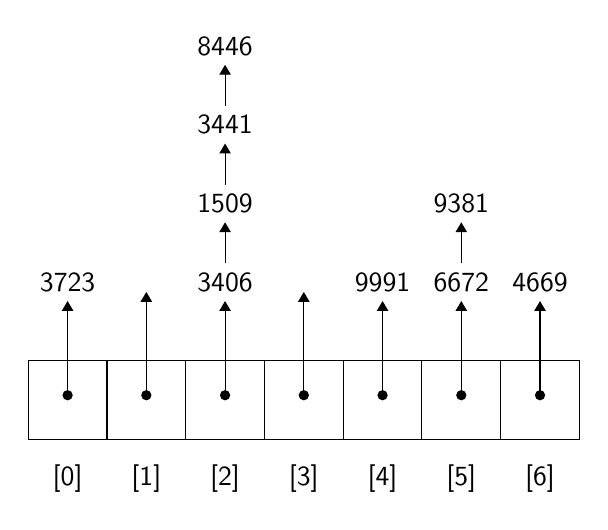
\begin{tikzpicture}[font=\sffamily,scale=0.5]
\draw (0, 0) rectangle (2, 2);
\draw (2, 0) rectangle (4, 2);
\draw (4, 0) rectangle (6, 2);
\draw (6, 0) rectangle (8, 2);
\draw (8, 0) rectangle (10, 2);
\draw (10, 0) rectangle (12, 2);
\draw (12, 0) rectangle (14, 2);
\draw (14, 0) rectangle (14, 2);
\node (0) at (1, -1) {[0]};
\node (1) at (3, -1) {[1]};
\node (2) at (5, -1) {[2]};
\node (3) at (7, -1) {[3]};
\node (4) at (9, -1) {[4]};
\node (5) at (11, -1) {[5]};
\node (6) at (13, -1) {[6]};
\node (a) at (1, 4) {3723};
\node (b) at (3, 4) {};
\node (c) at (5, 4) {3406};
\node (d) at (5, 6) {1509};
\node (e) at (7, 4) {};
\node (f) at (9, 4) {9991};
\node (g) at (11, 4) {6672};
\node (h) at (13, 4) {4669};
\node (i) at (5, 8) {3441};
\node (j) at (5, 10) {8446};
\node (k) at (11, 6) {9381};


\draw [Circle-Triangle] (1, 1) -- (a);
\draw [Circle-Triangle] (3, 1) -- (b);
\draw [Circle-Triangle] (5, 1) -- (c);
\draw [Circle-Triangle] (7, 1) -- (e);
\draw [Circle-Triangle] (9, 1) -- (f);
\draw [Circle-Triangle] (11, 1) -- (g);
\draw [Circle-Triangle] (13, 1) -- (h);
\draw [-Triangle] (c) -- (d);
\draw [-Triangle] (d) -- (i);
\draw [-Triangle] (i) -- (j);
\draw [-Triangle] (g) -- (k);
\end{tikzpicture}
\end{center}

\problem{2}
Based on the first question, we could find out there are 3 collisions, which is too many on index 2. So the table should be rehashed into another table whose size is a prime number and more than twice the original size. Thus, the size should be 17, which is twice more than 7 and is a prime number. And the hash function is $h(key)$ = 16 - ($key$ mod 17), which resulted the table as follows.
From the result follows, there are only 1 collision happened on index 2 and only 52.9$\%$ of the entries are occupied.



\begin{center}
% written for clarity, not for efficiency :)
% horizontal coordinates increase left to right
% vertical coordinates increase bottom to top
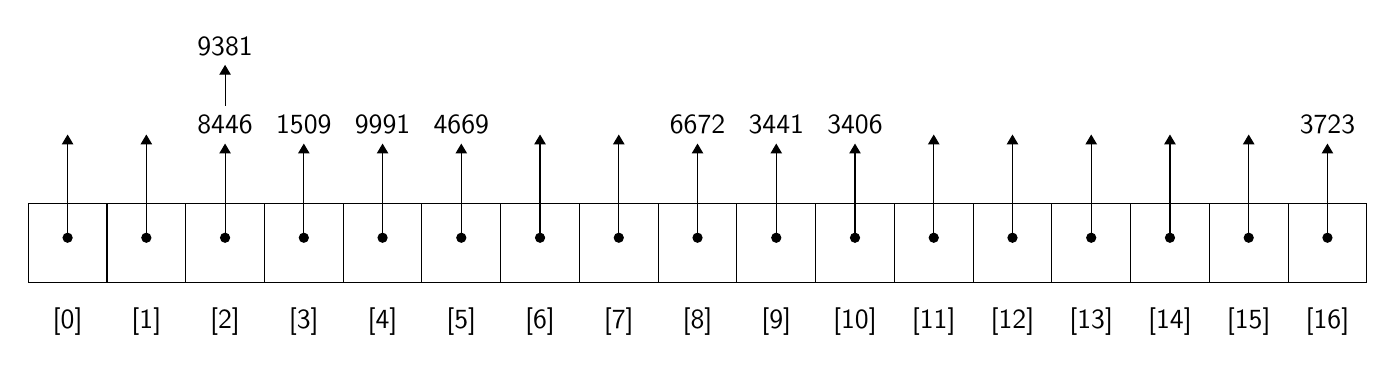
\begin{tikzpicture}[font=\sffamily,scale=0.5]

\draw (0, 0) rectangle (2, 2);
\draw (2, 0) rectangle (4, 2);
\draw (4, 0) rectangle (6, 2);
\draw (6, 0) rectangle (8, 2);
\draw (8, 0) rectangle (10, 2);
\draw (10, 0) rectangle (12, 2);
\draw (12, 0) rectangle (14, 2);
\draw (14, 0) rectangle (16, 2);
\draw (16, 0) rectangle (18, 2);
\draw (18, 0) rectangle (20, 2);
\draw (20, 0) rectangle (22, 2);
\draw (22, 0) rectangle (24, 2);
\draw (24, 0) rectangle (26, 2);
\draw (26, 0) rectangle (28, 2);
\draw (28, 0) rectangle (30, 2);
\draw (30, 0) rectangle (32, 2);
\draw (32, 0) rectangle (34, 2);

\node (0) at (1, -1) {[0]};
\node (1) at (3, -1) {[1]};
\node (2) at (5, -1) {[2]};
\node (3) at (7, -1) {[3]};
\node (4) at (9, -1) {[4]};
\node (5) at (11, -1) {[5]};
\node (6) at (13, -1) {[6]};
\node (7) at (15, -1) {[7]};
\node (8) at (17, -1) {[8]};
\node (9) at (19, -1) {[9]};
\node (10) at (21, -1) {[10]};
\node (11) at (23, -1) {[11]};
\node (12) at (25, -1) {[12]};
\node (13) at (27, -1) {[13]};
\node (14) at (29, -1) {[14]};
\node (15) at (31, -1) {[15]};
\node (16) at (33, -1) {[16]};


\node (a) at (1, 4) {};
\node (b) at (3, 4) {};
\node (c) at (5, 4) {8446};
\node (z) at (5, 6) {9381};
\node (d) at (7, 4) {1509};
\node (e) at (9, 4) {9991};
\node (f) at (11, 4) {4669};
\node (g) at (13, 4) {};
\node (h) at (15, 4) {};
\node (i) at (17, 4) {6672};
\node (j) at (19, 4) {3441};
\node (k) at (21, 4) {3406};
\node (l) at (23, 4) {};
\node (m) at (25, 4) {};
\node (n) at (27, 4) {};
\node (o) at (29, 4) {};
\node (p) at (31, 4) {};
\node (q) at (33, 4) {3723};

\draw [Circle-Triangle] (1, 1) -- (a);
\draw [Circle-Triangle] (3, 1) -- (b);
\draw [Circle-Triangle] (5, 1) -- (c);
\draw [Circle-Triangle] (7, 1) -- (d);
\draw [Circle-Triangle] (9, 1) -- (e);
\draw [Circle-Triangle] (11, 1) -- (f);
\draw [Circle-Triangle] (13, 1) -- (g);
\draw [Circle-Triangle] (15, 1) -- (h);
\draw [Circle-Triangle] (17, 1) -- (i);
\draw [Circle-Triangle] (19, 1) -- (j);
\draw [Circle-Triangle] (21, 1) -- (k);
\draw [Circle-Triangle] (23, 1) -- (l);
\draw [Circle-Triangle] (25, 1) -- (m);
\draw [Circle-Triangle] (27, 1) -- (n);
\draw [Circle-Triangle] (29, 1) -- (o);
\draw [Circle-Triangle] (31, 1) -- (p);
\draw [Circle-Triangle] (33, 1) -- (q);

\draw [-Triangle] (c) -- (z);

\end{tikzpicture}
\end{center}

\problem{3}
See the submitted file.
\newpage

\problem{4}\textit{Answer:}
Based on my code, the table size I chose is 102407. Which is the nearest and the prime number greater than 102401-the number of the words in the words file. The result I got is 37607 collisions. And the load factor is $\frac{102401}{102407}$ $\approx$ 0.9999414, which is most approximately equal to 1. The closer load factor approach to 1, the better performance the code could be.

\end{document}